% ---------------------------------------------------------------------------
\FloatBarrier
\section{Model Comparison and Prediction Horizon (RQ2, RQ4)}
\label{sec:models}

The paper uses one model family, a regularised linear model. This phase asks
whether other kinds of model do better with the same data (RQ2), whether the
F4 features also help them (RQ3, part 2), and how the error depends on the
number of early cycles used (RQ4). The code is in \texttt{src/pls.py},
\texttt{src/models.py}, \texttt{src/p4\_pls.py}, \texttt{src/p4\_models.py}
and \texttt{src/horizon.py}; \texttt{notebooks/04\_model\_comparison.ipynb}
shows every step.

\subsection{Choice of models and protocol}
The seven models planned in Section~\ref{sec:problem} were reduced to four
that suit 41 training cells and differ from the paper's in a specific way
(Table~\ref{tab:p4models}). Tree ensembles and neural networks were left out:
with this few cells they can memorise the training set, and trees cannot
predict outside the range of training lives, which matters for the
longest-lived cell (Section~\ref{sec:physics}).

\begin{table}[t]
\centering
\caption{Models compared in Phase~4. All predict $\log_{10}$(life) from
standardised inputs; settings are chosen on the training cells only.}
\label{tab:p4models}
\small
\setlength{\tabcolsep}{3pt}
\begin{tabular}{@{}>{\raggedright\arraybackslash}p{0.20\columnwidth}>{\raggedright\arraybackslash}p{0.40\columnwidth}>{\raggedright\arraybackslash}p{0.34\columnwidth}@{}}
\toprule
Model & Difference from the paper & Tuning \\
\midrule
PLS & uses the whole $\dq$ curve, not summary statistics & number of components, scaling; repeated 4-fold CV \\
Gaussian process (GP) & non-linear; gives a prediction interval & kernel by marginal likelihood (bounded, see text) \\
SVR (RBF kernel) & non-linear, robust loss & $C$, $\gamma$, $\varepsilon$; repeated 4-fold CV \\
Additive splines (GAM) & one smooth curve per feature & knots, ridge strength; repeated 4-fold CV \\
\bottomrule
\end{tabular}
\end{table}

Because every additional model evaluated on the same 40-odd test cells adds
a chance of a lucky result, the protocol of Phase~3 was kept. All model
variants, feature sets and settings were fixed using nested
cross-validation on the training cells; every registered configuration was
then evaluated once on the test sets and all are reported. The unseen batch
is not used (Phase~5). Scores are given as in Section~\ref{sec:physics}:
official RMSE and percentage error, the RMSE on test cells inside the
training life range, and paired bootstrap intervals against the elastic net
on identical cells inside that range.

One further feature was screened before the comparison, again on the
training cells only: the voltage drop of the discharge curve at fixed
charge between cycles 10 and 100, the ``vertical'' counterpart of $\dq$. It
correlates with $\log_{10}\mathrm{Var}(\dq)$ at $\rho=0.99$ and adds no
information ($-2.7$\,\% cross-validated gain, not significant within either
batch), so no new feature was added.

\subsection{PLS on the whole $\dq$ curve}
PLS compresses the curve (averaged into 100 voltage bins) into a few
weighted averages chosen to predict $\log_{10}$(life). Life follows a power
law in the $\dq$ amplitude, while PLS is linear in its inputs, so four input
versions were compared on the training cells (Table~\ref{tab:p4pls}): the
raw curve, the curve compressed with $\mathrm{asinh}(\Delta Q/1\,\mathrm{mAh})$
(logarithmic for large values), the amplitude $\log_{10}\mathrm{sd}(\dq)$ with the
shape $\dq/\mathrm{sd}(\dq)$ as two blocks, and F4 with the shape. In the
block versions each block is scaled to a share of the total variance chosen
by cross-validation; without this, one amplitude column is lost among 100
shape columns.

\begin{table}[t]
\centering
\caption{PLS variants and references: nested cross-validation RMSE of
$\log_{10}$(life) on the 41 training cells (identical folds).}
\label{tab:p4pls}
\begin{tabular}{@{}lc@{}}
\toprule
Model & RMSE $\log_{10}$ \\
\midrule
PLS, raw curve & 0.0892 \\
PLS, asinh curve & 0.0684 \\
PLS, amplitude + shape & 0.0706 \\
PLS, F4 + shape & 0.0543 \\
\midrule
Linear fit on $\log_{10}\mathrm{sd}(\dq)$ only & 0.0723 \\
Linear fit on F4 only & 0.0501 \\
Elastic net, F2 / F4 & 0.0578 / 0.0507 \\
\bottomrule
\end{tabular}
\end{table}

On the training cells the shape of the curve adds almost nothing beyond its
amplitude (0.0706 vs.\ 0.0723), and adding it to F4 makes the model worse
(0.0543 vs.\ 0.0501); when given both, cross-validation gives 90--99\,\% of the
variance to the F4 block.
This agrees with Section~\ref{sec:physics}, where the dQ/dV peak features
added nothing. The asinh curve, the best pure whole-curve model, and the F4 +
shape model were then evaluated once on the test sets. Neither beats the
elastic net on the primary set (128 and 152 cycles without the anomalous
cell, against 85 and 115), and both fail on the secondary set: 3431 cycles
for the asinh curve, with three cells (\texttt{b3c39}, \texttt{b3c16},
\texttt{b3c17}) predicted 9--12 times too long, and 285 for F4 + shape.

Fig.~\ref{fig:p4pls} shows why. The model places a large, narrow weight on
the voltage bins around 3.15\,V, the steep edge at the start of the plateau.
In the training batches this edge sits at almost the same voltage in every
cell, so small shifts in it appeared predictive. In the secondary batch the
edge lies at a different voltage ($\mathrm{asinh}\,\Delta Q$ of $-1.9$ instead of
$-3.0$ between 3.10 and 3.25\,V), which alone raises the predicted life by a
factor of about 2.2. The secondary batch differs in its procedure (5-second
rests, cells 3--4\,\textdegree C warmer at the start of the fast charge,
Table~\ref{tab:steps}), which plausibly shifts the plateau voltage under load.
A model that reads the whole curve thus finds narrow features that work
within the training batches but depend on the test procedure; the summary
statistics average over the whole plateau and are far more robust.

\begin{figure}[t]
  \centering
  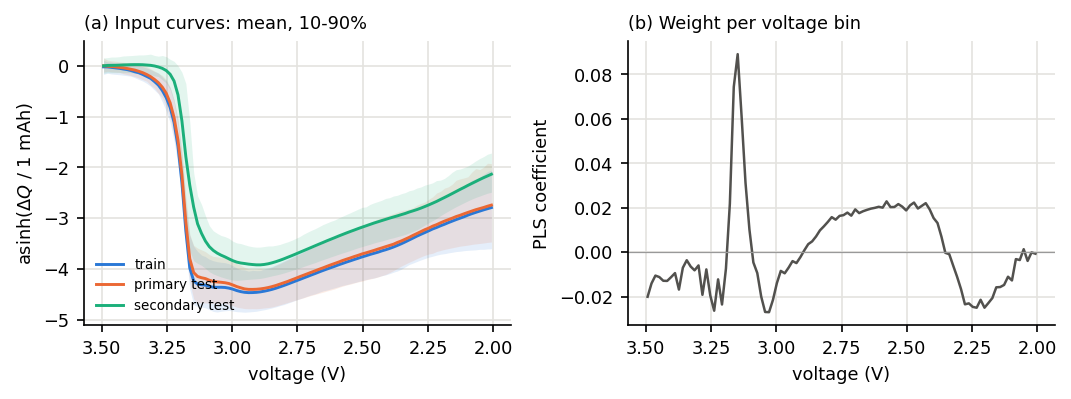
\includegraphics[width=\columnwidth]{fig_p4_pls}
  \caption{PLS on the whole curve. (a) Mean input curve (shaded: 10--90\,\%
  of cells) for each split. (b) Regression weight of each voltage bin; the
  peak near 3.15\,V lies where the secondary curves are shifted.}
  \label{fig:p4pls}
\end{figure}

\subsection{Gaussian process, SVR and additive splines}
The three models were each fitted to F2 (the paper's six discharge
features) and F4 (our two features). The GP kernel is a linear term plus a
Mat\'ern term with one length-scale per feature plus noise: log life is close
to linear in the log features, so the linear term carries the trend and lets
the model extrapolate, while the Mat\'ern term adds smooth deviations.
Without bounds, the GP interpolated the 41 training cells exactly (training
error zero). Two bounds were therefore set on the training cells: length-scales of at
least one standard deviation of each feature (equal or better nested CV for
both feature sets) and a noise floor of about a third of the elastic net's
cross-validated residual. The additive spline model extrapolates linearly
outside the training range.

\begin{table*}[t]
\centering
\caption{Test performance of all registered configurations: RMSE (cycles) /
mean percentage error. ``In range'': primary cells whose life lies inside the
training range (\texttt{b1c2} and \texttt{b2c1} removed). Bootstrap: change
in RMSE against the elastic net on the same features, on identical cells
inside the training range (95\,\% interval; negative = better). Bold:
interval excludes zero.}
\label{tab:p4test}
\small
\setlength{\tabcolsep}{3pt}
\begin{tabular}{@{}llccccccc@{}}
\toprule
Model & Set & CV ($\log_{10}$) & Primary & Prim.\ excl. & In range & Secondary & Boot.\ primary & Boot.\ secondary \\
\midrule
EN & F2 & 0.0578 & 90 / 12.6\,\% & 85 / 9.4\,\% & 86 & \textbf{167} / \textbf{9.9\,\%} & -- & -- \\
GP          & F2 & 0.0650 & \textbf{85} / 11.4\,\% & 79 / 8.1\,\% & 78 & 174 / 10.5\,\% & $-7$ [$-35$, $+19$] & $+8$ [$-4$, $+22$] \\
SVR         & F2 & 0.0677 & 176 / 12.6\,\% & 174 / 9.1\,\% & 65 & 169 / 9.7\,\% & $\mathbf{-20}$ [$-49$, $-3$] & $+1$ [$-9$, $+9$] \\
GAM         & F2 & 0.0776 & 242 / 10.6\,\% & 243 / 8.6\,\% & 79 & 169 / 14.5\,\% & $-8$ [$-28$, $+14$] & $+3$ [$-48$, $+58$] \\
\midrule
EN & F4 & 0.0507 & 114 / 9.9\,\% & 115 / 9.1\,\% & 75 & 170 / 11.1\,\% & -- & -- \\
GP          & F4 & \textbf{0.0478} & 103 / \textbf{7.9\,\%} & 103 / \textbf{6.6\,\%} & \textbf{64} & 180 / 11.4\,\% & $\mathbf{-11}$ [$-21$, $-3$] & $+9$ [$-1$, $+17$] \\
SVR         & F4 & 0.0576 & 107 / 9.3\,\% & 107 / 8.0\,\% & 76 & 190 / 14.9\,\% & $0$ [$-16$, $+17$] & $+22$ [$-15$, $+60$] \\
GAM         & F4 & 0.0593 & 92 / 8.3\,\% & 92 / 6.9\,\% & 66 & 207 / 16.3\,\% & $-10$ [$-24$, $+2$] & $+39$ [$-16$, $+95$] \\
\midrule
PLS         & curve & 0.0684 & 138 / 18.5\,\% & 128 / 12.9\,\% & 104 & 3431 / 99.2\,\% & $+14$ [$-25$, $+50$]$^\ast$ & $\mathbf{+3207}$ [$+467$, $+5094$]$^\ast$ \\
PLS         & F4+shape & 0.0543 & 151 / 10.5\,\% & 152 / 8.6\,\% & 117 & 285 / 21.7\,\% & $+34$ [$-21$, $+102$] & $\mathbf{+117}$ [$+28$, $+211$] \\
\bottomrule
\multicolumn{9}{@{}l}{\footnotesize EN: elastic net. $^\ast$ against the elastic net on F2.}
\end{tabular}
\end{table*}

Table~\ref{tab:p4test} and Fig.~\ref{fig:p4models} give the results. Three
patterns stand out.

\textbf{Within the training batches the non-linear models help.} On the
primary cells inside the training range, the GP on F4 (64 cycles), SVR on F2
(65) and the spline model on F4 (66) all beat the elastic net (75--86). Two of
these gains are resolved by the bootstrap: GP-F4 by 11 cycles and SVR-F2 by 20.

\textbf{On the new batch they do not.} On the secondary set no
configuration is significantly better than the elastic net, and the more
flexible ones are worse (spline model on F4: 207 vs.\ 170). The extra
flexibility captures relations specific to the two training batches, which
is the same lesson as for PLS and for the batch-proxy features of
Section~\ref{sec:physics}.

\textbf{Models without a linear backbone break outside the training range.}
Table~\ref{tab:p4extrap} lists the two primary cells whose lives lie outside
the training range. SVR falls back towards the training average and the
spline model bends the wrong way, so for SVR-F2 and GAM-F2 these two cells
cause 87--90\,\% of the primary squared error, which explains their official
primary RMSE of 176 and 242. The elastic net and the GP, whose linear kernel
term extrapolates, stay sensible.

\begin{table}[t]
\centering
\caption{Predictions for the two primary-test cells outside the training
life range (300--2160 cycles).}
\label{tab:p4extrap}
\begin{tabular}{@{}lcc@{}}
\toprule
Model & \texttt{b1c2} (2237) & \texttt{b2c1} (148) \\
\midrule
Elastic net F2 / F4 & 2192 / 1667 & 360 / 212 \\
GP F2 / F4 & 2341 / 1708 & 367 / 243 \\
SVR F2 / F4 & 1186 / 1741 & 388 / 244 \\
GAM F2 / F4 & 742 / 1820 & 291 / 246 \\
\bottomrule
\end{tabular}
\end{table}

\begin{figure}[t]
  \centering
  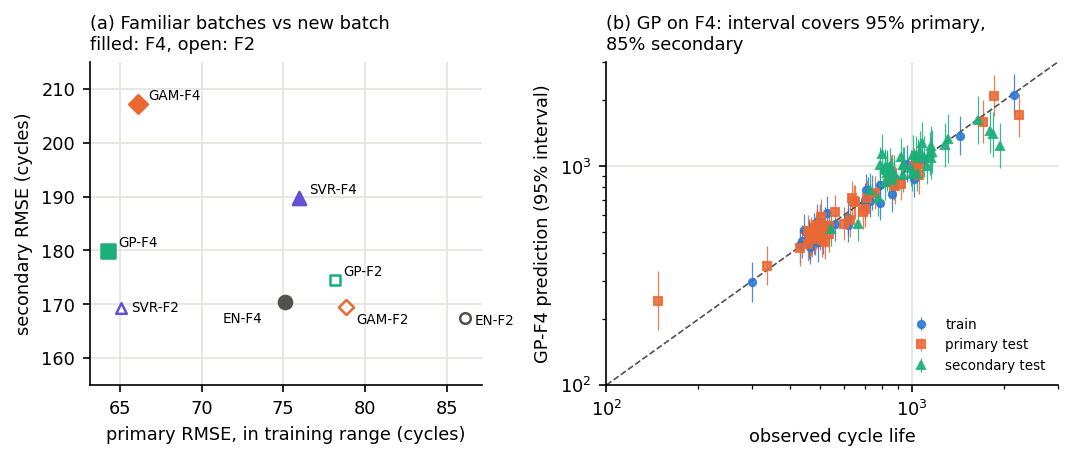
\includegraphics[width=\columnwidth]{fig_p4_models}
  \caption{(a) RMSE on the primary cells inside the training range against
  RMSE on the secondary set, for every configuration (PLS lies off the scale:
  secondary 285 and 3431). (b) GP on F4: predictions with 95\,\% intervals.}
  \label{fig:p4models}
\end{figure}

\textbf{Uncertainty.} The GP on F4 gives well-calibrated 95\,\% intervals on
the primary set (95\,\% of the cells inside; typical width a factor of 1.20)
but is overconfident on the secondary set (85\,\%): it does not know that the
procedure changed. The GP on F2 widens its interval for \texttt{b1c2}
(factor 1.84 against 1.16 typically), so it does flag that cell, but it still
nearly interpolates the training cells (training RMSE 10 cycles) and covers
only 81\,\% of the primary cells.

\subsection{Number of early cycles (RQ4)}
All features were recomputed from cycles $\le N$ ($\dq=Q_N(V)-Q_{10}(V)$,
fits and minima over cycles 2--$N$, IR($N$)$-$IR(2)), for $N$ from 20 to 150,
and every model was re-tuned on the training cells at each $N$. For $N=150$
the cache was extended to 160 cycles; all features at $N=100$ are unchanged.
\texttt{b2c1}, which reaches end of life at cycle 148, is excluded from the
primary scores at every $N$. Table~\ref{tab:p4horizon} and
Fig.~\ref{fig:p4horizon} show the results.

\begin{table*}[t]
\centering
\caption{Test RMSE (cycles) against the number of early cycles $N$:
primary set without \texttt{b2c1} / secondary set. Life used: median share of
a cell's life consumed by cycle $N$. Constant baseline: 399 / 511.}
\label{tab:p4horizon}
\begin{tabular}{@{}lcccccccc@{}}
\toprule
$N$ & 20 & 30 & 40 & 50 & 60 & 80 & 100 & 150 \\
Life used & 3\,\% & 4\,\% & 5\,\% & 7\,\% & 8\,\% & 11\,\% & 14\,\% & 20\,\% \\
\midrule
Elastic net F2 & 399 / 511 & 306 / 350 & 191 / 182 & 1829 / 1186 & 428 / 439 & 169 / 209 & 85 / 167 & 82 / 199 \\
Elastic net F3 & 233 / 396 & 205 / 345 & 157 / 212 & 168 / 247 & 142 / 230 & 146 / 213 & 122 / 220 & 103 / 224 \\
Elastic net F4 & 399 / 511 & 309 / 304 & 202 / 252 & 186 / 255 & 218 / 238 & 208 / 223 & 115 / 170 & 114 / 177 \\
GP F4 & 357 / 428 & 311 / 298 & 202 / 248 & 167 / 270 & 203 / 260 & 190 / 221 & 103 / 180 & 82 / 194 \\
\bottomrule
\end{tabular}
\end{table*}

\begin{figure}[t]
  \centering
  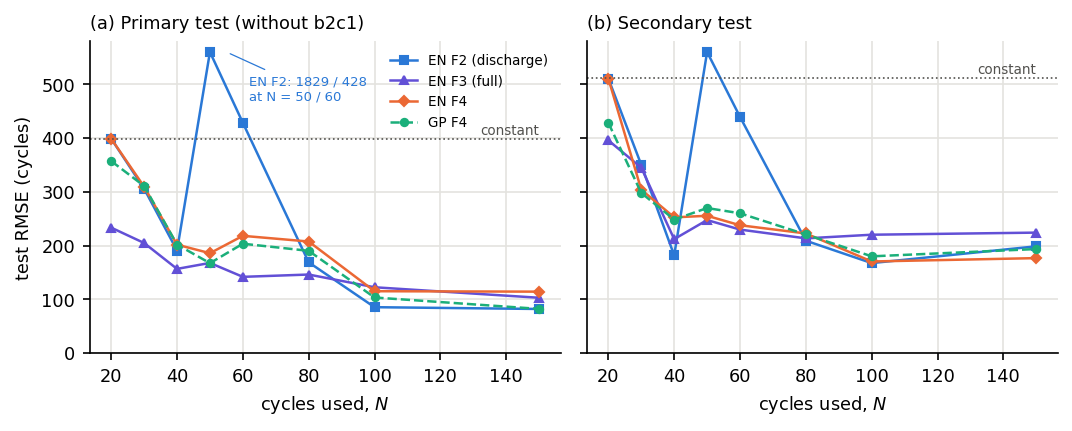
\includegraphics[width=\columnwidth]{fig_p4_horizon}
  \caption{Test RMSE against the number of early cycles $N$ (values above
  560 cycles clipped). Dotted: constant baseline.}
  \label{fig:p4horizon}
\end{figure}

\begin{itemize}
  \item \textbf{Below about 30 cycles $\dq$ carries no signal.} At $N=20$ the
  elastic net on F2 and F4 sets every weight to zero and returns the constant
  baseline; $\dq_{20-10}$ is mostly noise and the overhang rise. Only the full
  model (F3) predicts well that early, because charge time, temperature
  integral and IR are available from cycle 2. They describe the charging
  policy and the batch rather than the cell, and on the secondary set their
  advantage largely disappears (396 vs.\ 511).
  \item \textbf{From 40 to 80 cycles} (5--11\,\% of life) every model reaches
  roughly half the error of the constant baseline.
  \item \textbf{Between 80 and 100 cycles the error drops clearly} (e.g.\
  elastic net F2 169 to 85, F4 208 to 115); on the secondary set the
  improvement is significant for both. Part of this may be because the
  paper's features and F4 were designed at $N=100$.
  \item \textbf{Beyond 100 cycles nothing is gained.} From 100 to 150 cycles no
  model improves significantly; the GP on F4 gets significantly worse on the
  secondary set (+14 cycles) and the others do not change significantly.
  The rate measured by $\dq$ grows linearly (Section~\ref{sec:physics}), so
  cycle 150 adds signal the model does not need, while short-lived cells
  begin to leave the early regime.
  \item \textbf{The paper's log-of-absolute-value features are fragile early
  on.} At $N=50$ the elastic net on F2 predicts a life of 13\,393 cycles for
  \texttt{b1c0}: its $\dq_{50-10}$ is still close to zero, so
  $\log_{10}|\min\dq|$ lies 8.7 standard deviations outside the training
  range. F4 uses a standard deviation, which cannot pass through zero, and
  has no such failure.
  \item \textbf{GP vs.\ elastic net on F4 across $N$.} The GP is better on the
  primary set at most horizons (significantly at $N=60$, 100 and 150) and equal
  or worse on the secondary set (significantly worse at $N=60$ and 150).
  The exception is $N=20$, where the elastic net returns the constant and the
  GP is better on both sets (and $N=40$, where it is 4 cycles better on the
  secondary set).
\end{itemize}

\subsection{Answers}
\textbf{RQ2.} With 41 training cells, no model beats the paper's
regularised linear model on a new batch. Non-linear models (GP, SVR, additive
splines) are better within the training batches, significantly so for two of
them, but equal or worse on the secondary batch; models without a linear
backbone fail for lives outside the training range; and PLS on the whole
$\dq$ curve fails on the new batch because it relies on narrow,
procedure-dependent features. The most useful alternative is the GP on F4,
which is the best model within the training batches and gives calibrated
uncertainty there.

\textbf{RQ3, part 2.} With every model type except SVR, F4 gives the best
within-batch result of the two feature sets (GP 64, spline model 66, elastic net
75 cycles); on the new batch F2 remains slightly better.

\textbf{RQ4.} About 40 cycles (5\,\% of life) suffice for a rough screen at
half the error of the constant baseline; 100 cycles are clearly better; more
than 100 cycles bring no gain. Below 30 cycles only information about the
charging policy and batch helps.

\textbf{Caveats.} Eight new configurations were evaluated on the same
primary and secondary sets (Table~\ref{tab:p4test}), in addition to the five
of Sections~\ref{sec:reproduction} and~\ref{sec:physics}, and the horizon
study adds five models at eight values of $N$. Only differences whose
bootstrap interval excludes zero should be relied on, and even those carry
some multiple-comparison optimism. The secondary set
is a single batch, so ``new batch'' means one specific change of procedure;
Phase~5 tests the same models on a second unseen batch.
